% Chapter X

\chapter{Infection through the lense of genomics} % Chapter title

\label{ch:01-02} % For referencing the chapter elsewhere, use \autoref{ch:name} 

%----------------------------------------------------------------------------------------

Discoveries in biology are typically associated with progresses and advances in technological development, and the toolbox to detect and investigate bacterial infection traditionally included biochemical assays and microscopy. The recent advances in DNA sequencing have spurred a rapid extension of sequencing-derived, genomewide methods. Here we introduce the different ways these genomics approaches can provide biological insights into the biology of bacterial pathogens.

\section{Pathogen characterization}

A key task related to infection in biomedical research is the detection and characterization of infectious agents. This is of public health relevance, as it allows to test patients presenting suspicious symptoms for the presence of known pathogens, or determine the pathogenicity of a particular strain. 

Genotyping, i.e. the determination of one sample's genetic make-up from DNA analysis, can be achieved using molecular biology techniques such as \acrfull{RFLP} or \acrfull{PFGE} \cite{ochoa-diazBacterialGenotypingMethods2018}. These techniques use gel electrophoresis, which relies on the negative charges carried by DNA molecules. When put in a polymer gel submitted to an electromagnetic field, these acidic molecules migrate along the electrical current towards the positive pole of the field. The migration distance depends on the density of the gel polymer meshwork that impairs progression of DNA, and is proportional to the size of DNA molecules. After migration is complete, the gel can be treated with chemical reagent such as ethidium bromide, a fluorescent agent that intercalates between bases pairs. These treatments allow to highlight the position of DNA molecules. A large DNA molecule can be fragmented using a \Gls{restriction enzyme} into smaller segments of sizes able to migrate in the gel. Those will generate discrete bands of similar-length DNA fragments once revealed by chemical reagents. Together these bands form a bar-code of the larger molecule, and can be interpreted by the scientist to draw conclusions about its presence or nature. In the case of \acrshort{RFLP}, the entire genome is digested by restriction enzymes beforehand. The digestion will result in a series of discrete fragments whose lengths can be seen on the gel. Bacterial genotypes have different mutations which will affect the digestion pattern and resulting barcode on the gel.

While these methods work well to determine differences between alleles, they do not inform us on the actual DNA sequence involved. The advent of DNA sequencing made it possible to directly link phenotype with associated sequences of nucleotides. In theory, \acrfull{WGS}, the process of determining the nucleotide sequence of an entire genome at a single time, provides accurate information on an organism's nucleotidic or structural polymorphisms compared to the genome sequences of related strains, allowing to define genotypes at a finer scale. The main shortcoming of \acrshort{WGS} is its higher cost than other genotyping techniques, but the recent plummeting of sequencing costs have made it relatively affordable. These advantages have made \acrshort{WGS} a popular approach in clinical settings.

\section{Genomics to probe homeostasis}

When host cells are exposed to or infected by a pathogen, their homeostatic state is disrupted. This disruption is a combination of alterations caused by the pathogen to colonize the host cell and host-triggered immune reactions to improve its survival. Multiple levels of regulation are affected upon infection, from signalling to epigenetic modifications \cite{rolandoLegionellaPneumophilaType2014}. Over the years, a vast arsenal of NGS techniques has been developed to characterize and investigate these regulatory states. 

The most widely used approach consists in gene expression analysis (RNA-seq). The total transcribed RNAs present in a biological sample made of cells (infected or not) can be extracted, and reverse-transcribed into cDNA. That cDNA can be then sequenced and the relative abundance of each gene's transcript determined. This allows to quantify the expression of the whole genome, known as the transcriptome. Typical transcriptome analysis consists in comparing different conditions, to find out which genes undergo perturbations (increase or decrease of expression levels) during infection. 

Many levels of regulation allow to fine tune gene expression in eukaryotes (Fig. \ref{fig:01-02:transcriptional-regulation}). Regulatory elements encoded in the sequence, such as enhancers, can trigger or facilitate the recruitment of protein complexes to modulate gene expression \cite{levoPursuitDesignPrinciples2014}. Regulation can also apply at the post-translational level, for example by degrading proteins \cite{brownSREBPPathwayRegulation1997} or applying chemical modifications such as phosphorylation or acetylation to modulate their activity \cite{christensenPosttranslationalProteinAcetylation2019}. Epigenetic changes, in the form of chemical modification of histone proteins offer yet another way to regulate gene expression in eukaryotes. These chemical modifications are thought to collectively form a "histone code" \cite{strahlLanguageCovalentHistone2000} - a combinatorial set of instructions dictating the regulatory state of DNA sequences. Although the role of many histone modifications is still partially or completely unknown, there are many examples of histone marks affecting chromatin structure \cite{huangPredictingChromatinOrganization2015,wangHistoneModificationsRegulate2019} and gene transcription (Tab. \ref{tab:histones}). The amount of epigenetic marks can be quantified along the genome using another NGS-derived technique known as \acrfull{ChIPseq}. In \acrshort{ChIPseq}, the chromatin sample is crosslinked with formaldehyde, a fixative molecule that will generate covalent bonds between proteins and DNA. The sample is then sonicated to break the DNA into smaller fragments. Beads coated with antibodies targeted against a protein of interest (e.g. an epigenetic mark) are then used to precipitate and isolate DNA molecules bound to the protein of interest from the pool of total DNA. The crosslink is then reversed and the DNA fragments purified. This allows to retrieve all genomic regions that were bound to the protein of interest. 

\begin{figure}
    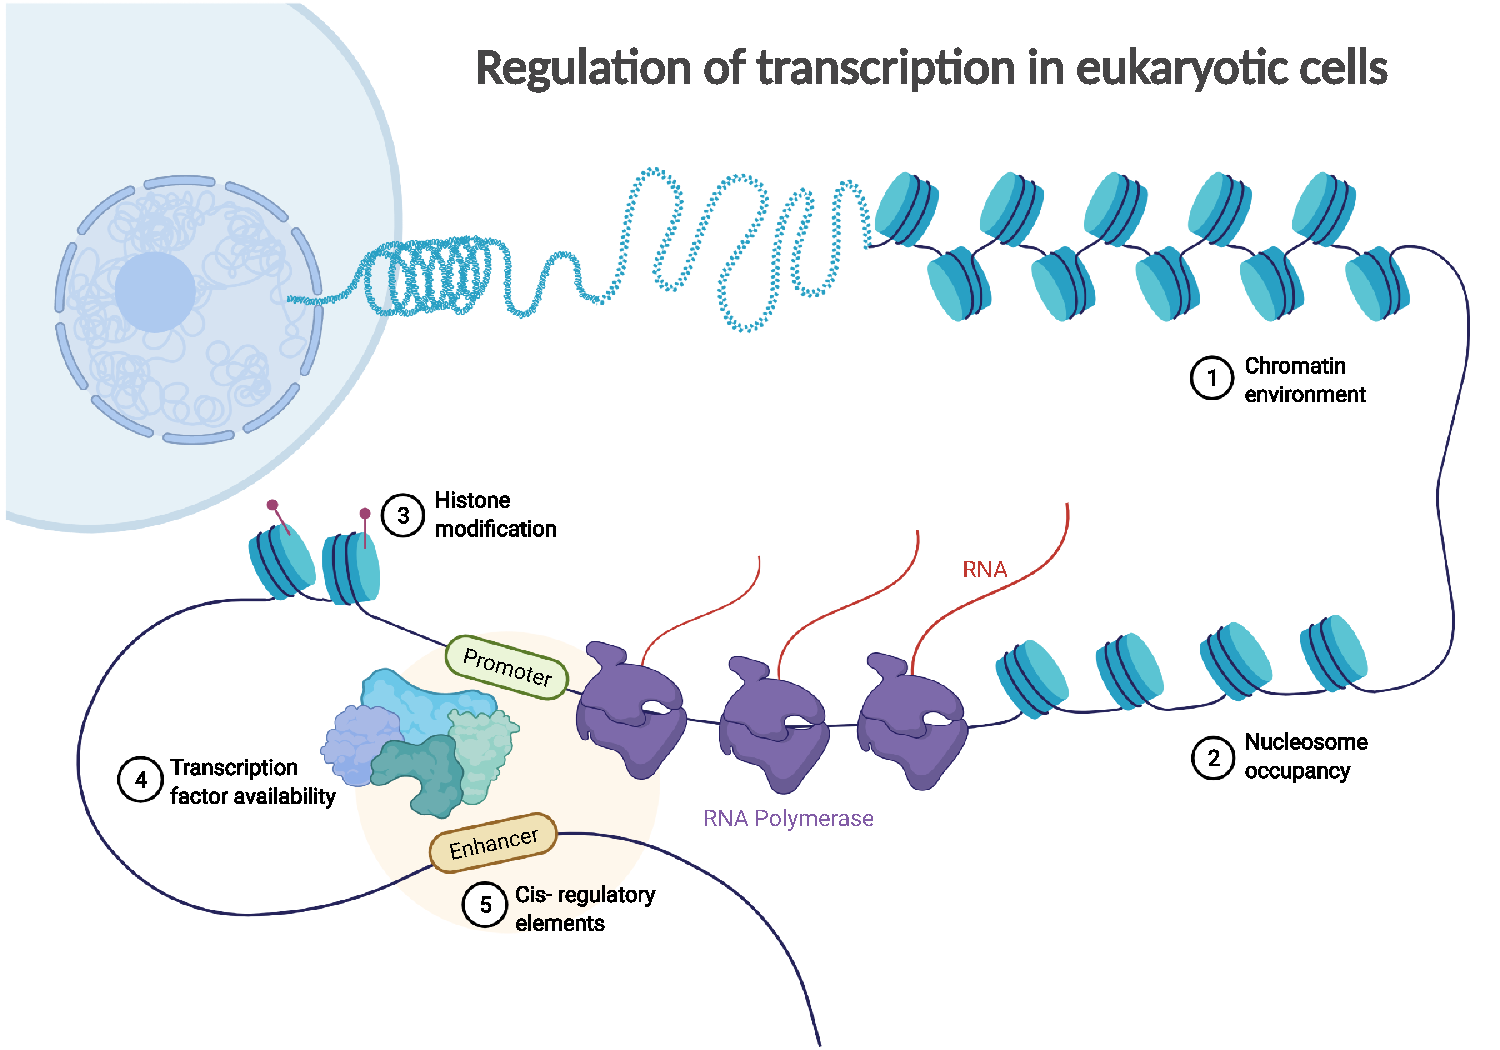
\includegraphics[width=\textwidth]{Parts/Part01/gfx/transcriptional_regulation_levels.pdf}
    \caption[Regulation of transcription in eukaryotic cells.]{Regulation of transcription in eukaryotic cells. Visual summary of the different levels at which transcription can be regulated. At the largest scale (1), the chromatin environment can form structures affecting transcription. The open space between nucleosome can also affect accessibility of protein complexes to gene sequences (2). Chemical modifications on histone proteins form an epigenetic code defining the recruitment of transcriptional complexes on the genome (3). The availability of those factors (4) and the proximity of regulatory sequences such as enhancers (5) provide another level of transcriptional regulation. Reprinted from “Regulation of Transcription in Eukaryotic Cells”, by BioRender.com (2020). Retrieved from https://app.biorender.com/biorender-templates }
    \label{fig:01-02:transcriptional-regulation}
\end{figure}

\begin{table}[]
\begin{tabularx}{\textwidth}{l | X | l | l}
\topline
\headcol Mark     & Regulatory state             & Type          & Sources \\ \midline
         H3K4Me1  & primed enhancers             & active        & \cite{benevolenskayaHistoneH3K4Demethylases2007}                                  \\
\rowcol  H3K4Me3  & active promoters             & active        & \cite{liangDistinctLocalizationHistone2004,kochLandscapeHistoneModifications2007} \\
         H3K9Me2  & facultative heterochromatin  & repressive    & \cite{poleshkoH3K9me2OrchestratesInheritance2019}                                 \\
\rowcol  H3K9Me3  & constitutive heterochromatin & repressive    & \cite{rosenfeldDeterminationEnrichedHistone2009}                                  \\
         H3K27Me3 & repressed genes              & repressive    & \cite{barskiHighResolutionProfilingHistone2007}                                   \\
\rowcol  H3K27Ac  & active enhancers             & active        & \cite{creyghtonHistoneH3K27acSeparates2010}                                       \\
         H3K36Me3 & transcribed gene bodies      & active        & \cite{kolasinska-zwierzDifferentialChromatinMarking2009}                          \\
\hline
\end{tabularx}
\caption[Example of regulatory histone marks]{Examples of commonly studied histone modifications of Histone subunit 3 and their impact on transcriptional regulation.}
\label{tab:histones}
\end{table}

\section{Capturing chromosome conformation}

Most eukaryotic chromosomes are made of a linear DNA molecule which is not randomly organized into the nuclear space. This long polymer can fold back on itself, resulting in three-dimensional structures which have several useful properties. One of the of most obvious, direct advantages of folding consists in compactness: for example, the human chromosome 1 is made of 250 millions nucleotides, each spaced by 0.34\si{\nano\meter} \cite {langridgeMolecularConfigurationDeoxyribonucleic1960}. If straightened, the chromosome would be 85\si{\milli\meter} long, yet the whole genome fits into a nucleus of $\sim$10\si{\micro\meter} in diameter. Another benefit of genome folding lies in its potential to contribute to the regulation of gene expression through the formation of multi-scale structures \cite{bonevOrganizationFunction3D2016}. Compacting large regions of the genome by spreading of \Gls{heterochromatin} allows to repress their activity \cite{gilbertChromatinArchitectureHuman2004}. Smaller scale structures, such as chromatin loops, appear also involved in the fine tuning of gene regulation \cite{bonevOrganizationFunction3D2016}. For example, it is suspected that such \Gls{chromatin} loops play a role in bridging enhancers and promoters, even though these sequences can be separated by large genomic distances \cite{doyleChromatinLoopsAllosteric2014,dowenMultipleStructuralMaintenance2013,dorsettCohesinActiveGenes2013}. Chromatin can also organize into compact self-interacting neighbourhoods forming local "domains", with distinct domains being isolated from each other. Here too, the significance of such local structures remains relatively elusive, and is being investigated in a number of Eukaryotic species. In mammals, \acrfull{TAD}s are also associated with large scale, cohesin-dependent loops \cite{ji3DChromosomeRegulatory2016}, while in other species such as the budding yeast and fruit fly, self-interacting domains could be more delimited by supercoiling, as they display highly expressed genes at their extremities \cite{hsiehMappingNucleosomeResolution2015,chathothChromatinArchitectureReorganization2019}. Transcription \textit{per se} could therefore be a direct player of chromosome folding, but the reciprocal interplay between transcription and folding remains also elusive and investigated. Nevertheless, characterizing the regulation of these different levels of chromosome folding is an essential step towards understanding their potential interplay with chromosome function, including the coordination of the gene expression program with other cellular processes.

\subsection{3C technologies}

The use of genomics to investigate the 3D folding of genomes started with the invention of the \acrfull{3C} technique \cite{dekkerCapturingChromosomeConformation2002}. This technique allowed to quantify the relative frequencies of physical contacts between pairs of DNA segments in a genome (Fig. \ref{fig:01-02:3c}, left). This is done by crosslinking the genome with formaldehyde, a small chemical fixative molecule that forms stable bonds between DNA and proteins, and subsequently digesting the genome with a restriction enzyme. Genomic regions closer in space will be crosslinked together more frequently. Performed over a population of cells, this will result in DNA-protein complexes, where chromatin fragments from genomic regions that were on average spatially closer to each other will be over-represented compared to DNA segments that were on average more distant from each other. A DNA ligase is then added to the mix, resulting in the ligation of DNA segments, with a strong bias towards segments that have been trapped together within the same DNA-protein complex. As a result, on average, DNA segments that were closer to each other will be preferentially ligated together compared to segments distant from each other in the population of cells. The crosslink is then reversed. In the original 3C protocol, the relative frequency of religation events between segments of interest (i.e. presumed to reflect their relative contact frequency, hence spatial proximity) was assessed using semi-quantitative \acrshort{PCR}. Primers designed to hybridize on two regions of interest were used to perform a semi-qPCR. Quantified onto a gel, the amount of amplified product, once normalized, reflected the relative contact frequency of two known genomic loci. Some limitations of the technique are the requirement to select regions to monitor and the design of qPCR oligonucleotides, which could also lead to a number of biases and caveats. Nevertheless, 3C was successfully used in the seminal study by Dekker et al. \cite{dekkerCapturingChromosomeConformation2002} to characterize the overall conformation of budding yeast chromosome III from a 12 x 12 contact map (reflecting the number of qPCR primers designed). This contact map was further converted into a distance matrix, itself useful to generate a 3D representation of the chromosome. These remarkable data remained fully consistent over the next two decades with results obtained using improved protocols offering increasingly high resolutions. 

\begin{figure}[htb]
    \centering
    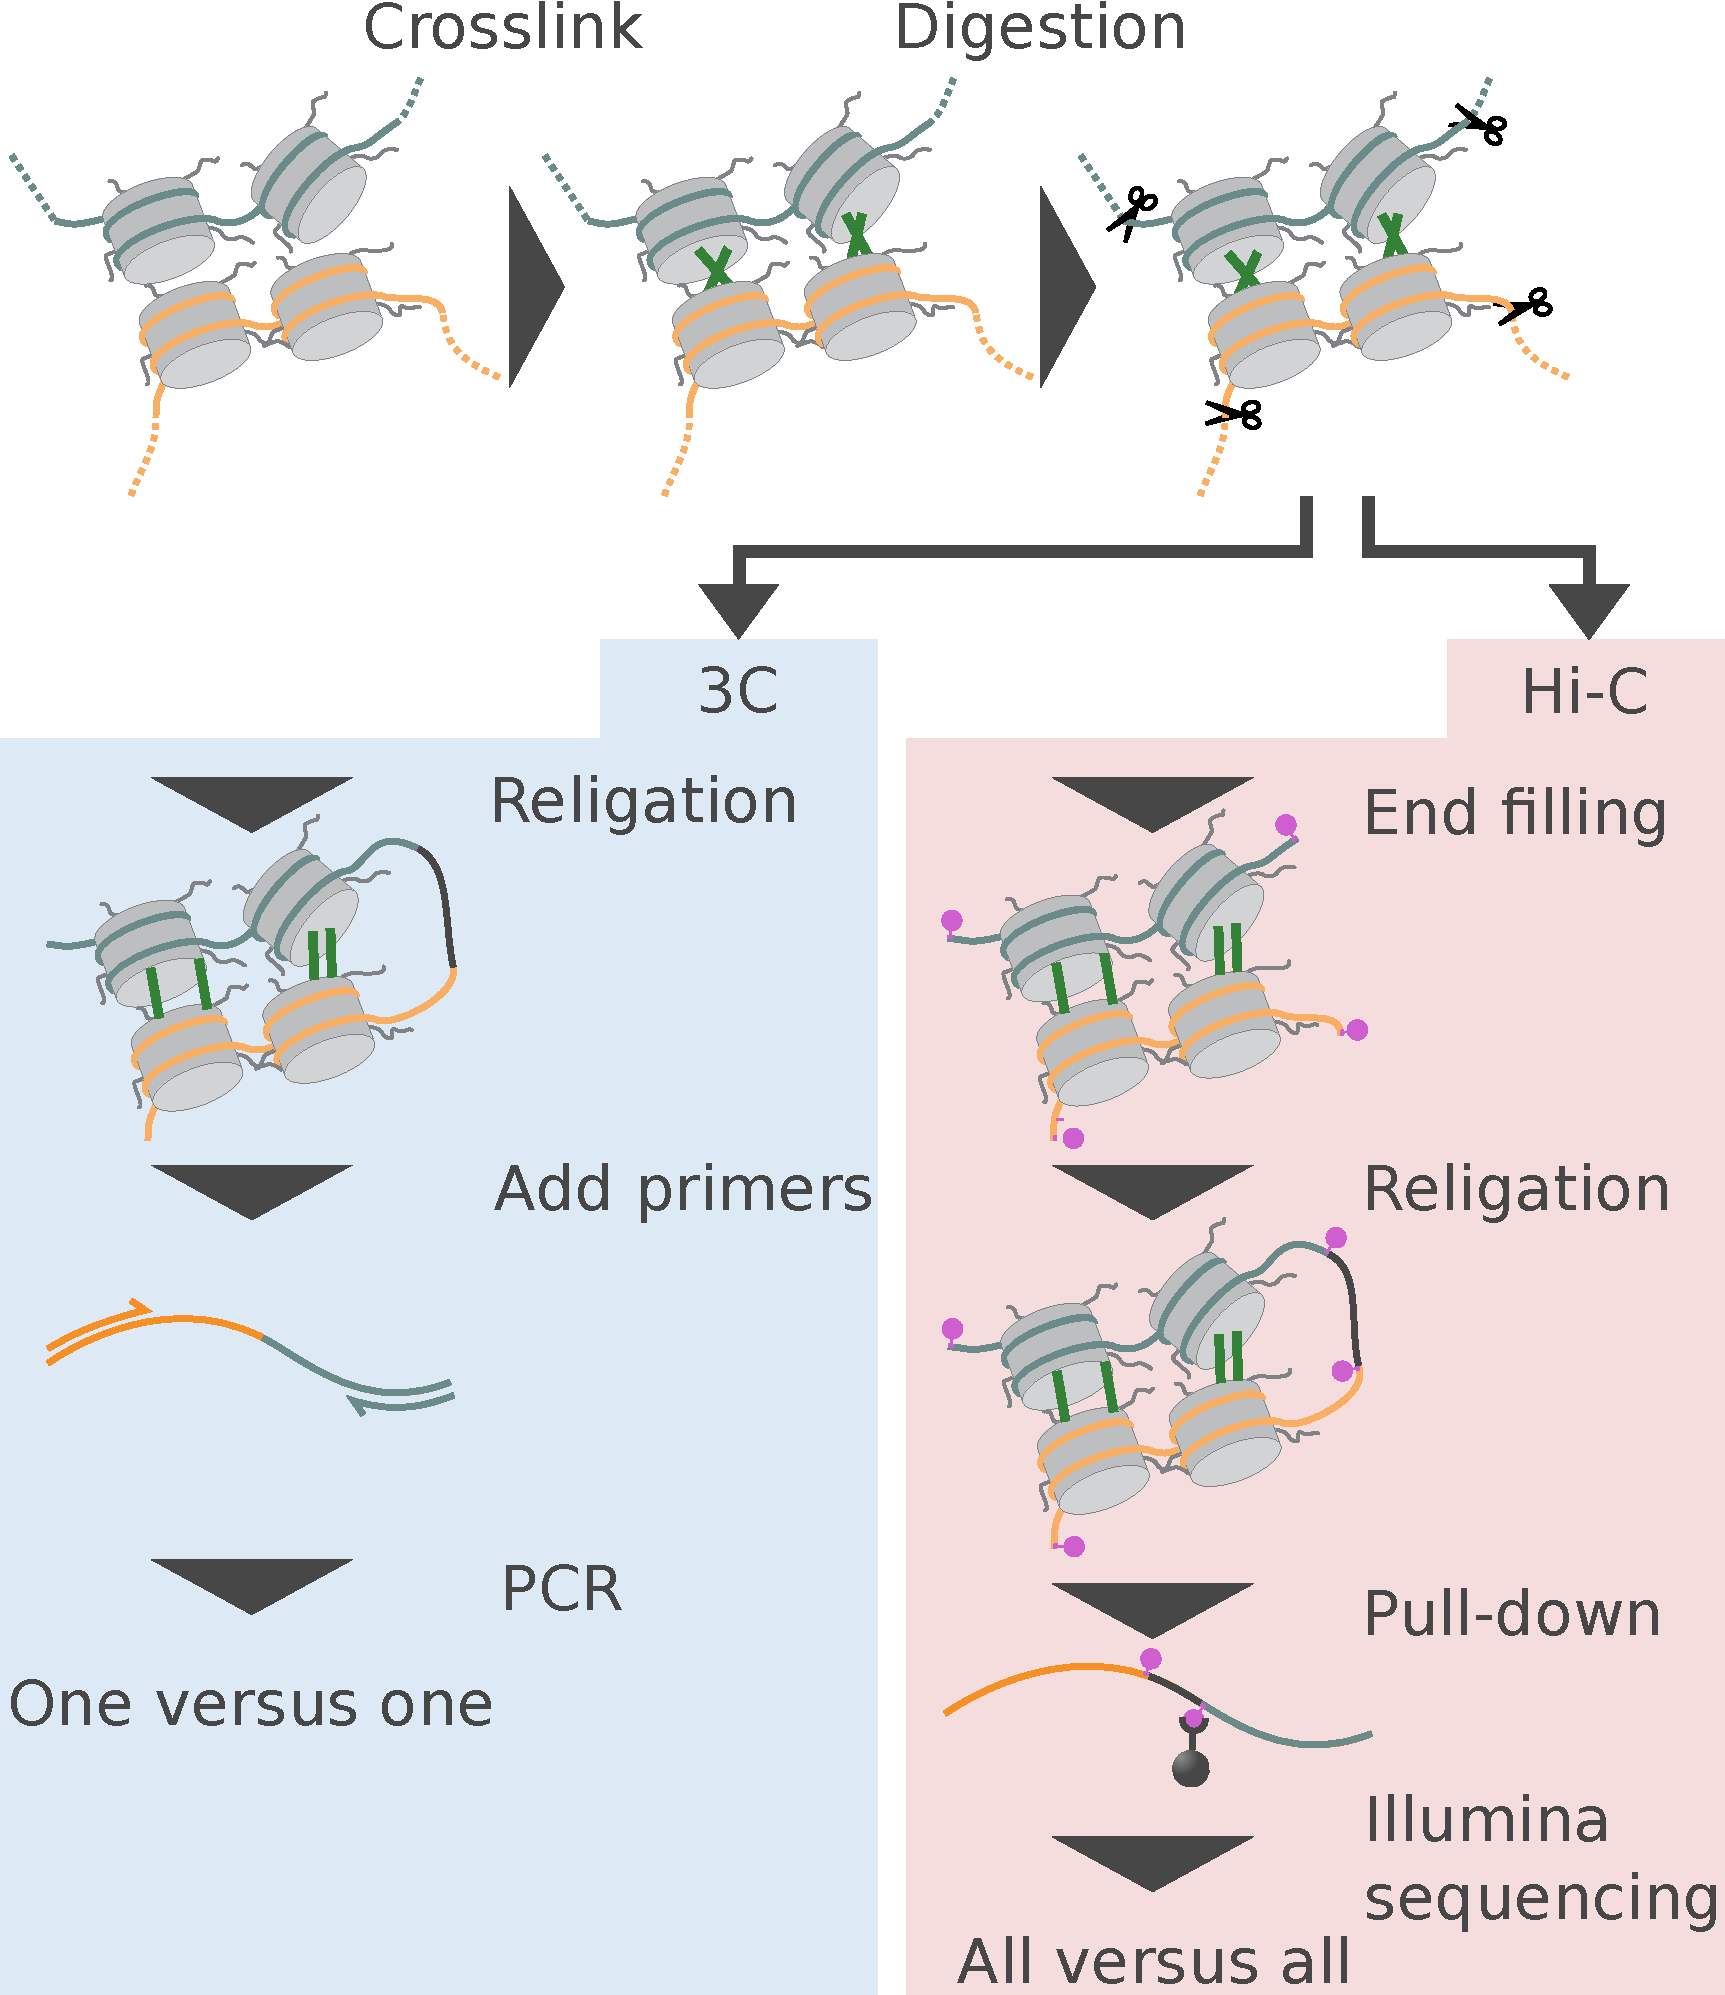
\includegraphics[width=0.7\textwidth]{Parts/Part01/gfx/3c_protocol.pdf}
    \caption[Chromosome conformation capture protocol.]{Chromosome conformation capture protocol: Chromosome conformation capture protocols share common steps (top): The chromatin is first crosslinked to form covalent DNA-protein bonds and then digested using a restriction enzyme. The Hi-C protocol subsequently differs from the original 3C protocol. In 3C (left), fragments are religated, the crosslinked is reversed and specific primers are added to amplify a pair of known loci. This allows to quantify interaction between 2 loci. In Hi-C (right), the fragments ends are filled with biotinylated nucleotides (pink), religated and the crosslinked is reversed. Streptavidin beads are then used to pull down religation products which are then sequenced.}
	\label{fig:01-02:3c}
\end{figure}

From then on, many derivatives of the \acrshort{3C} technique were developed. The most significant improvement was enabled by the possibility to perform paired-end high-throughput sequencing, which led to the development of a genome-wide application of 3C, called Hi-C (Fig. \ref{fig:01-02:3c}, right). This method shares the main steps of 3C, the main difference being that pair-end sequencing is used instead of qPCR. In Hi-C, fragment ends are filled with biotin prior to religation \cite{lieberman-aidenComprehensiveMappingLongRange2009} and religated products are enriched through pull-down using streptavidin beads (which have high affinity for biotin). After ligation, sequencing primers are directly plugged to the extremities of the 3C enriched library. Paired-end sequencing is performed, and each read of the pair is then aligned onto the reference genome to determine its original position. This procedure allows to quantify the contact frequency of all versus all loci in the genome instead of using specific primers for a single pair of loci. 

The information generated by Hi-C experiments therefore consists in counting how many times pairs of restriction fragments were found ligated together. This results in a list of contacts between all (in theory) pairs of restriction fragments in a genome. These contacts are most commonly visualized and interpreted using matrices, also called contact maps (Fig. \ref{fig:01-02:hic}a), which are two-entry tables represented as color-coded heat maps. The color of each value in the matrix corresponds to its value relative to the others, reflecting the contact frequency between the associated pair of fragments. Those contact maps are an indirect representation of the presumed tri-dimensional folding of chromosomes. When processed and associated with other "omics" data, or performed in various mutant contexts, they are rich in information regarding chromosome regulation.

The various folding structures formed by chromatin can result from the direct or indirect action of DNA binding proteins. In mammals (and most metazoans), a typical example is the CCCTC-binding factor \acrfull{CTCF}, a transcription factor that also appears to act as an "architectural protein" structuring chromatin. Molecular motors such as the members of the \acrfull{SMC} complexes (cohesin, condensin...) and other proteins families slide along DNA to operate various roles. When cohesin is loaded onto the chromosome, it can extrude two strands of DNA in opposite directions through its ring-shaped structure, a process known as loop extrusion \cite{fudenbergFormationChromosomalDomains2016}. When cohesin encounters a roadblock protein such as \acrshort{CTCF} the extrusion stops, forming a chromatin loop and maintaining contact between the two DNA strands. Depending on the location of those roadblocks, this can form stable interactions between distant genomic regions. 

%%% ROMAIN STOPPED HERE %%%

Each spatial structure formed by chromatin is reflected on the contact map as a distinct pattern (Fig. \ref{fig:01-02:hic}b). At the largest scale, chromosomes are isolated from each other in the nucleus, occupying distinct "chromosome territories". This is reflected as dark squares along the diagonal of the whole genome contact map as each chromosome interacts more with itself than any other chromosome (Fig. \ref{fig:01-02:hic}a). Within each chromosome chromatin forms "insulation domains", known as \acrfull{TAD} in mammals. Genes sharing the same domain are in close proximity, while being isolated from genes in neighbouring domains . Genes within the same domain also tend to be co-regulated \cite{noraSpatialPartitioningRegulatory2012}. Domains form dark squares along the diagonal of a chromosome, due to the enriched intra-domain interactions at the expense of inter-domain contacts (Fig. \ref{fig:01-02:hic}b, bottom). At a finer scale, chromatin loops are visible on contact maps as dots away from the diagonal (Fig. \ref{fig:01-02:hic}b, middle). The coordinates of those dots correspond to the genomic positions of roadblocks which stopped the extrusion process.



\begin{figure}[htb]
    \centering
    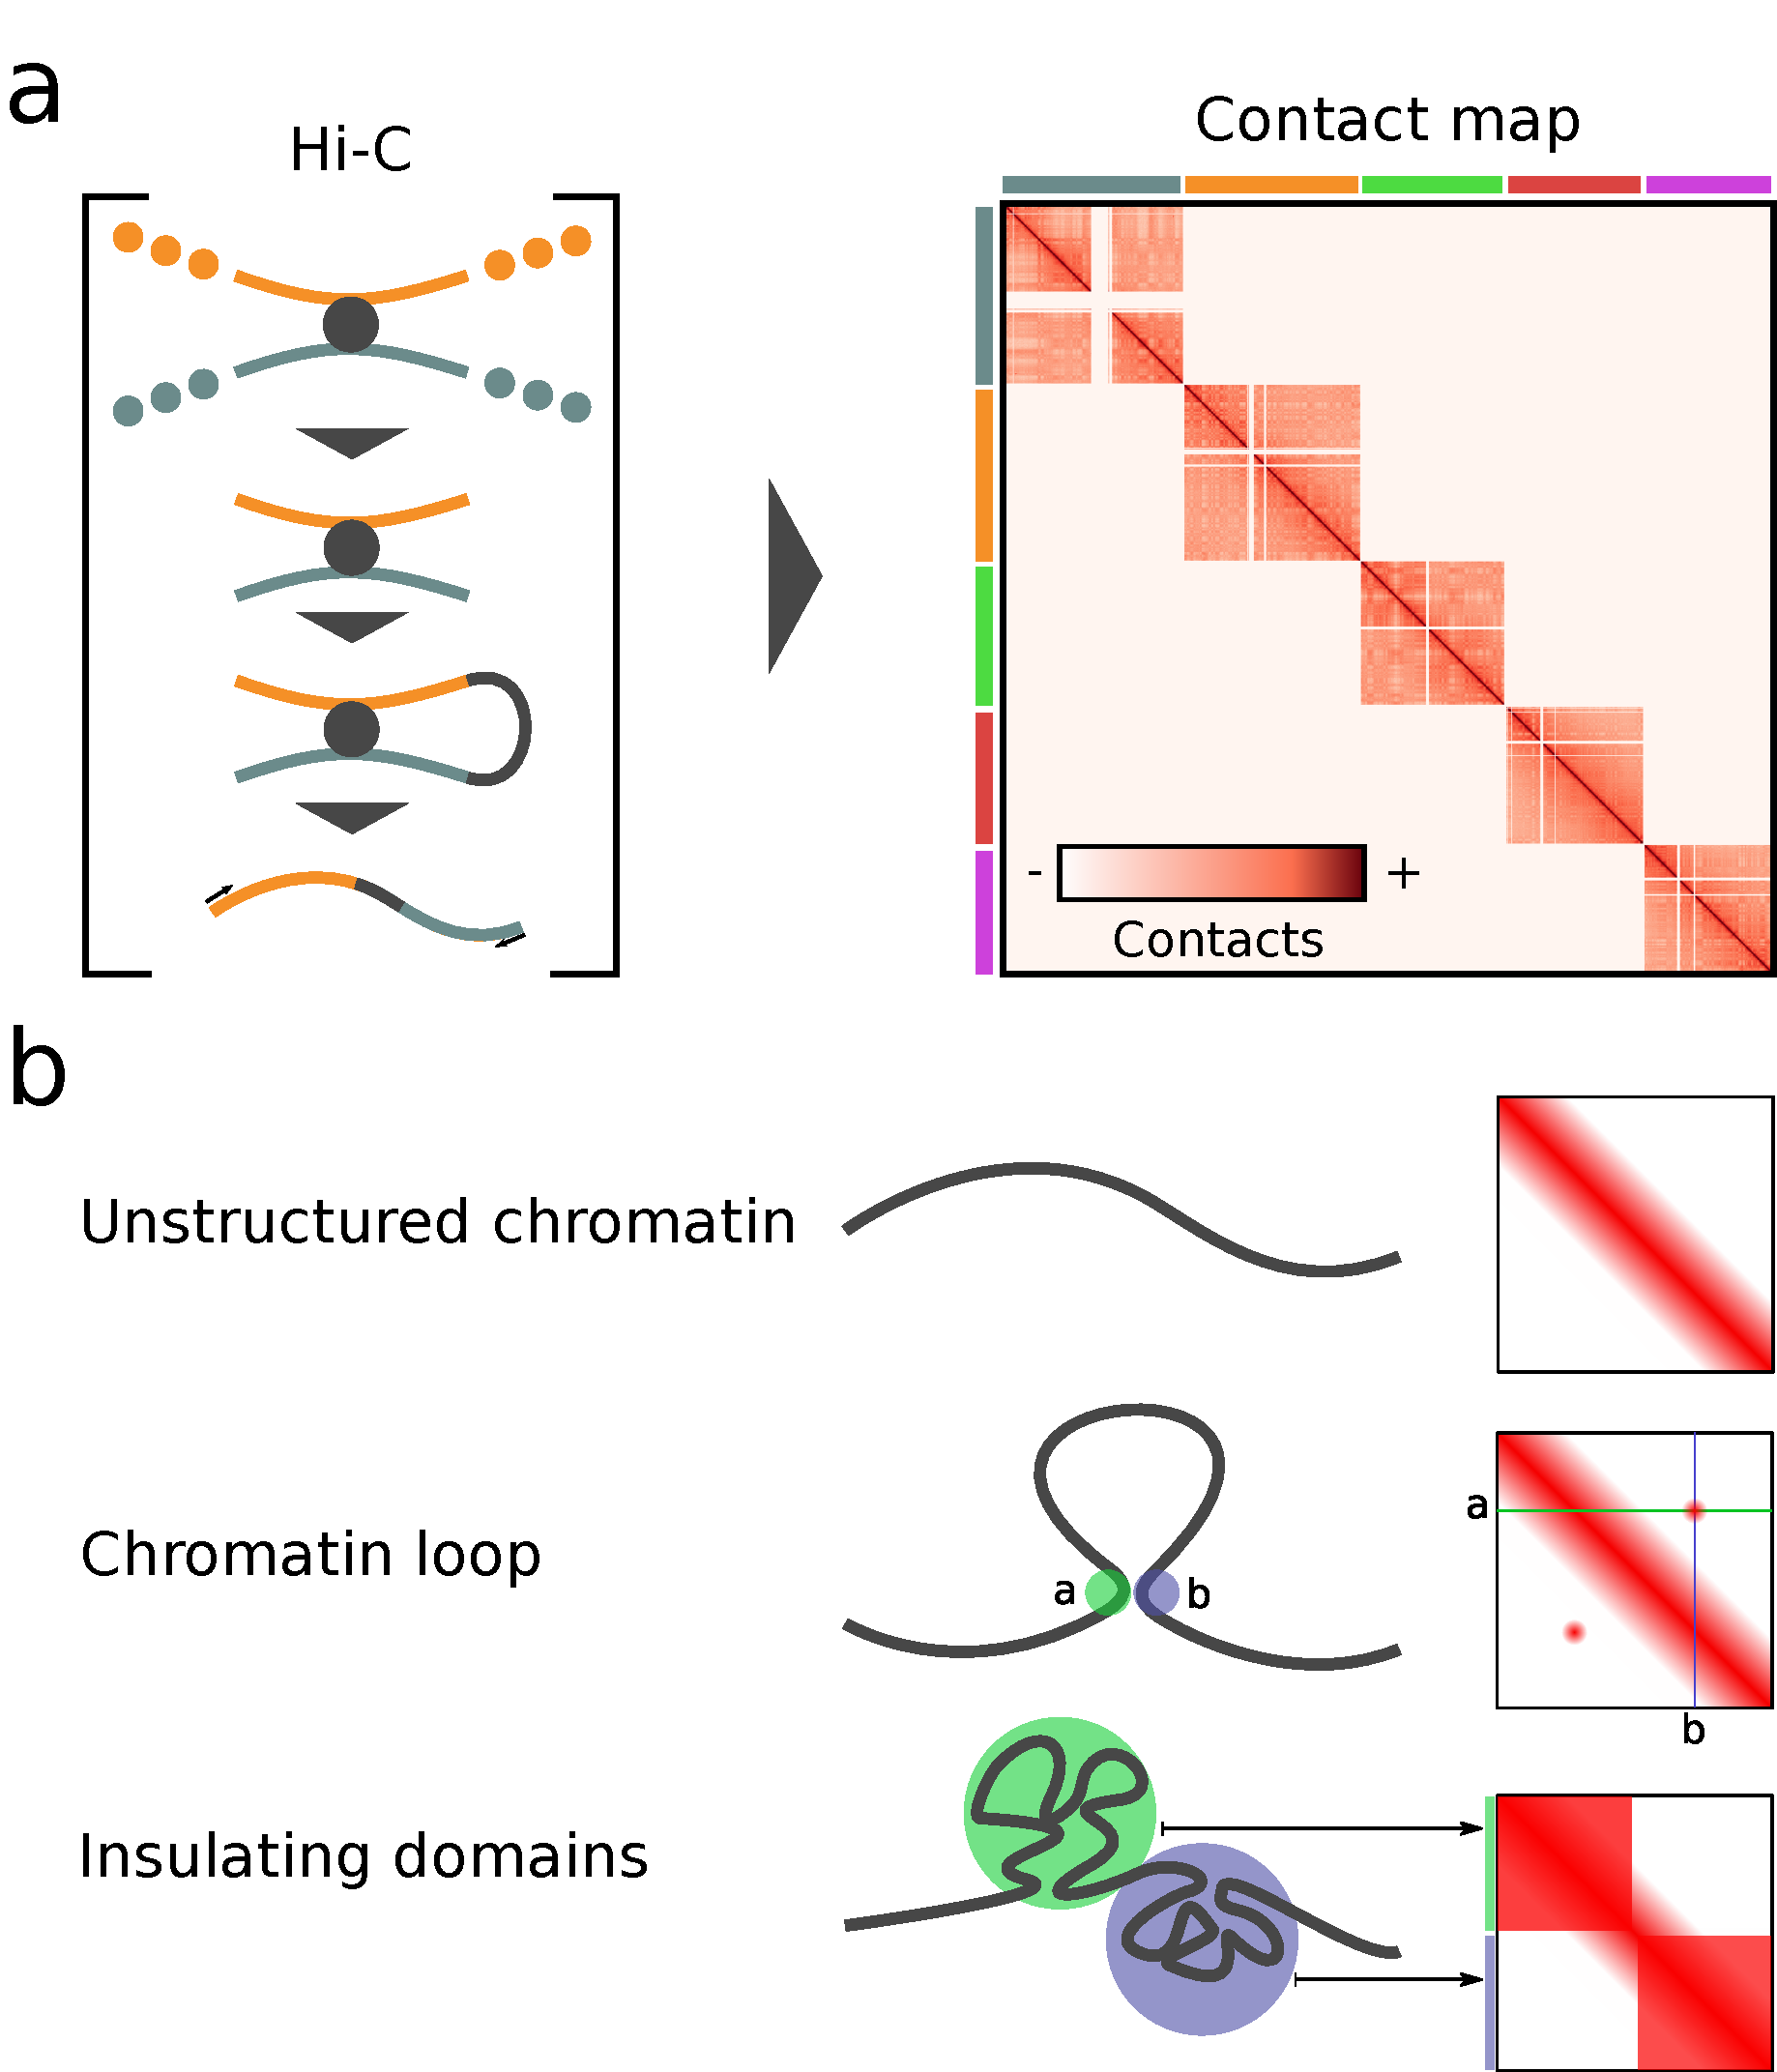
\includegraphics[width=0.7\textwidth]{Parts/Part01/gfx/hic_interpretation.pdf}
    \caption[Interpretation of Hi-C contact maps.]{Interpretation of Hi-C contact maps: \textbf{a}: The Hi-C protocol (left) generates millions of read pairs representing contacts between genomic loci in a population of cells. Those contacts can be stored into an all-versus-all contact matrix (right) averaging all contacts in the population. Each chromosome in the matrix forms a square of strong self-interactions along the diagonal due to chromosomal territories. \textbf{b:} Within each chromosomal map, different contact patterns reflect specific conformations (right). The main feature of a contact map is the diagonal gradient (top) caused by the contact decay according to genomic distances. Chromatin loops between two anchor loci are visible as dots away from the diagonal (middle). Insulation domains form squares along the diagonal of a chromosome where loci within the same domain interact strongly, but interactions between domains are depleted.}
	\label{fig:01-02:hic}
\end{figure}

In many eukaryotes, chromatin is also segregated into active and inactive compartments, commonly known as "euchromatin" and "heterochromatin" or A/B compartments. The A (active) compartment has higher GC content, gene density and gene expression than its counterpart \cite{lieberman-aidenComprehensiveMappingLongRange2009}. A and B compartments also occupy separate spaces in the nucleus; whereas the A compartment is located towards the middle of the nucleus, the B compartment is relegated to the nuclear periphery and associated with lamina domains \cite{vansteenselLaminaAssociatedDomainsLinks2017}. This spatial segregation results in preferential physical interactions within the same compartment, which are reflected on Hi-C contact maps by a plaid-like pattern. 

\subsection{Analysis of chromosome contact maps}

The most visible element on any chromosome contact map is the diagonal gradient reflecting the power-law relationship between genomic distance and contact frequency. This is often called the distance-decay function or $P(s)$ where $s$ means genomic distance and $P$ probability of contacts. The slope of the $P(s)$ in itself holds information on the relative contribution of short range and long range contacts in the chromosome, which is linked to chromosome compaction.

Due to the high intensity of this gradient, other patterns of biological relevance are often obscured on the contact map. A common preprocessing step to account for it is to apply an \acrfull{o/e} normalization of the Hi-C map, where each pixel is divided by the average of its diagonal (Fig. \ref{fig:01-02:compartments}a). Lower intensity patterns such as domains, compartments and chromatin loops are easier to perceive on the resulting map.

After \acrshort{o/e} normalization, the compartment signal is generally the most salient feature on the contact maps. It can be extracted using \acrfull{PCA} on the normalized contact map \cite{lajoieHitchhikerGuideHiC2015} and retrieving the first few eigenvectors (i.e. principal component) explaining the most variance (Fig. \ref{fig:01-02:compartments}b). In some cases where the compartment signal is weak (e.g. noisy datasets), it may not be contained in the first eigenvector. A robust approach is to select the eigenvector with the strongest absolute correlation to an external signal known to be associated with active chromatin, such as gene expression or GC content \cite{sergeyvenevOpen2cCooltoolsV02021} (Fig. \ref{fig:01-02:compartments}c). The sign of the eigenvector is arbitrary, and it must be "phased" with the feature by flipping its sign to ensure a positive correlation with the said feature. In the phased vector, regions in the A compartment will contain positive values and \textit{vice versa}. The positions at which the sign changes are boundaries between different compartments (Fig. \ref{fig:01-02:compartments}d).

\begin{figure}[h!]
    \centering
    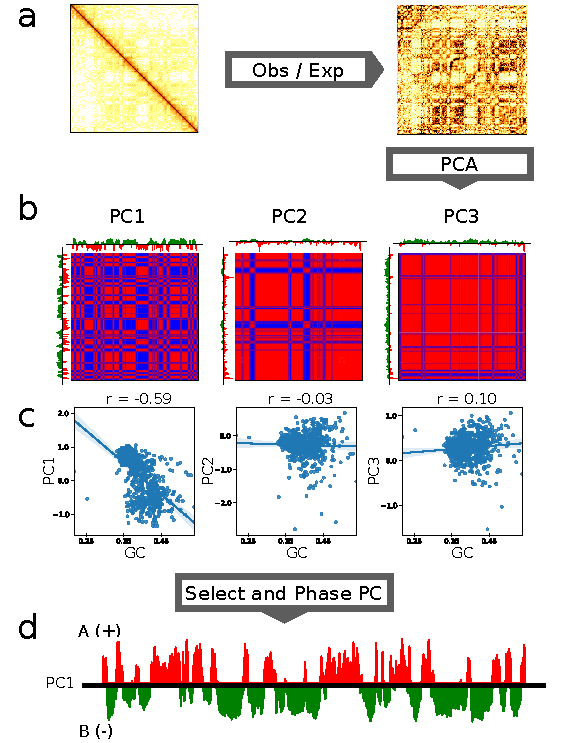
\includegraphics[width=0.90\textwidth]{Parts/Part01/gfx/hic_pca_compartments.pdf}
    \caption[Representation and analysis of chromatin compartments in Hi-C.]{Representation and analysis of chromatin compartments in Hi-C. \textbf{a:} \acrfull{o/e} normalization is applied to the balanced contact map to remove the distance-decay gradient. Higher frequency of interactions within the same compartment result in a plaid-like pattern on chromosome contact maps. \textbf{b:} PCA is applied to the \acrshort{o/e} normalized contact map and the first few principal components (PC) are retained. For visualization, each PC is shown alongside its outer product, yielding the rank-1 reconstruction of the contact map. The outer product matrix is binarized (negative=blue, positive=red) to show the compartmentalization. \textbf{c:} The correlation of each PC with GC content is computed, to select the PC with the highest absolute correlation. \textbf{d:} The sign of PCs being meaningless, the selected PC is phased (by changing its sign in case of negative correlation) to ensure positive values represent A compartment.}
    \label{fig:01-02:compartments}
\end{figure}

Many genomes are segmented into \acrshort{TAD}s containing frequently interacting loci, and often co-regulated genes. Regions in separate \acrshort{TAD}s are insulated from each other, and the strength of this insulation can be quantified using an "insulation score". The insulation score of a given region is defined as the intensity of contacts across that region (upstream with downstream) \cite{craneCondensindrivenRemodellingChromosome2015} and can be represented as a numerical track along the genome. Improved metrics such as the relative insulation score have since been developed to successfully detect \acrshort{TAD}s \cite{chenHiCDBSensitiveRobust2018}. The relative insulation score (RI) at a locus \textit{s} between bins \textit{k} and \textit{k+1} with a predetermined window size \textit{w} is defined as:

\begin{align}
    \label{eqn:01-02:insulation-U}
    U(w, s) &= \sum_{i=-w}^{-1}{\sum_{j=0}^{i+1}{M_{k+i,k+j}}} \\
    \label{eqn:01-02:insulation-D}
    D(w, s) &= \sum_{i=-w+1}^{0}{\sum_{j=1}^{w+i}{M_{k+i,k+j}}} \\
    \label{eqn:01-02:insulation-B}
    B(w, s) &= \sum_{i=1}^{w}{\sum_{j=i+1}^{w+1}{M_{k+i,k+j}}} \\
    \label{eqn:01-02:insulation-RI}
    RI(w, s) &= \frac{U(w, s) + D(w, s) - B(w, s)}{U(w, s) + D(w, s) + B(w, s)}
\end{align}

Where U and D are contacts in the upstream and downstream regions respectively, and B are the contacts between U and D. This can be visually represented as a triangle sliding along the diagonal of the Hi-C matrix (Fig. \ref{fig:01-02:insulation}). By contrast the original insulation score consisted only in computing B (Eq. \ref{eqn:01-02:insulation-B}).

\begin{figure}[htb]
    \centering
    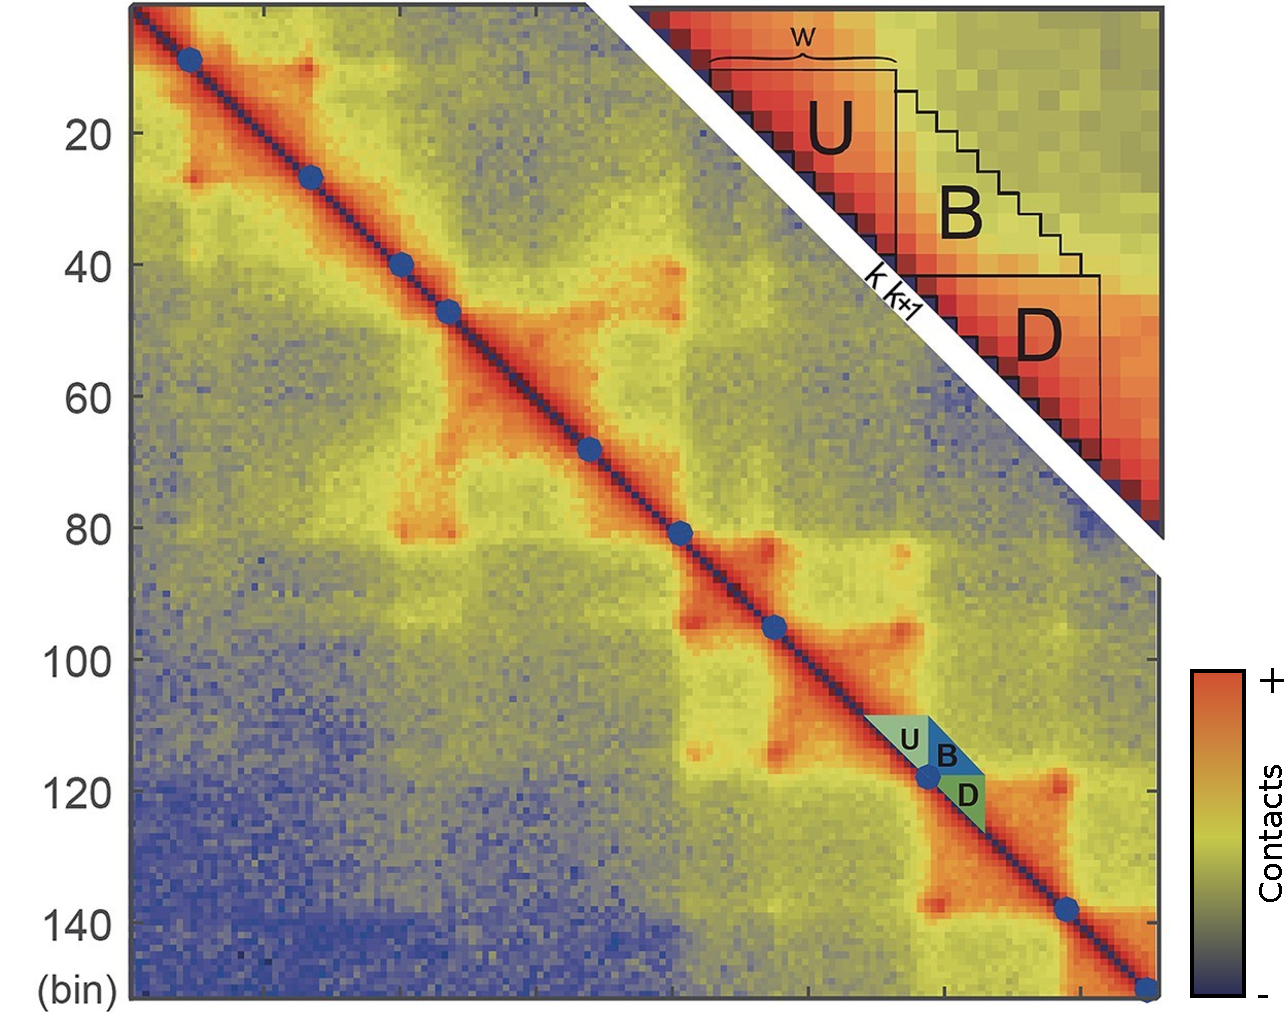
\includegraphics[width=0.8\textwidth]{Parts/Part01/gfx/insulation_score_hicdb.pdf}
    \caption[Visual illustration of the relative insulation score.]{Visual illustration of the relative insulation score. Computing the relative insulation score at bin k involves computing the average interactions between upstream (U) and downstream (D) regions, denoted as B, as well as the average contacts within U and B. The key parameter when computing insulation is the window size (w), determining the size of the U, B and D. Figure adapted from \cite{chenHiCDBSensitiveRobust2018}}
    \label{fig:01-02:insulation}
\end{figure}


At a smaller scale than \acrshort{TAD}s, chromatin loops contain valuable information about interactions between regulatory elements. Some tools detect these loops by searching for local enrichment of contacts, appearing as dots away from the diagonal \citep{durandJuiceboxProvidesVisualization2016,ramirezHighresolutionTADsReveal2018}. However, current loop detection algorithms suffer from low detection rates (recall). As such, an alternative approach is to focus on a set of genomic intervals of interest (e.g. binding sites of a transcription factor) and compute a window average of all pairs of intervals. The resulting average, often called pile-up, can be used to visualize the presence of chromatin loops between regions, or be compared between mutants \cite{flyamerCoolpupPyVersatile2020}.

Quantifying contact changes is useful in the study of many biological processes, such as differentiation or cell cycle progression. In that regard, the most global comparison, is to compute a similarity metric between pairs of samples. This is also useful as quality control, to estimate technical (replicates) and biological (conditions) variability. Different comparison metrics have been used, such as the sum of differences between Hi-C matrices \cite{ursuGenomeDISCOConcordanceScore2018}, correlation coefficients \cite{yangHiCRepAssessingReproducibility} or distance between the matrix eigenvectors \cite{yanHiCspectorMatrixLibrary2017}.

Rather than computing a single metric for each sample, most applications of Hi-C require the identification of regions where the chromatin behaviour changes. Several methods aiming to achieve this are adapted from existing count-based algorithms designed for RNA-seq \citep{lunDiffHicBioconductorPackage2015,stansfieldMultiHiCcompareJointNormalization2019,heinzSimpleCombinationsLineageDetermining2010}. In this analogy, they consider each bin of the genome as a "gene" and their contacts as an expression count. A discrete probability distribution is then fitted to the bin counts and used to identify bins with significant contact changes consistant across replicates. This approach relies on solid statistical grounds, but it often does not address the question at hand. Often times, when analysing Hi-C data, we are interested in finding specific structures appearing or disappearing rather than a simple contact change at a region. The development of methods to discover relevant changes in chromatin conformation is still an active area of research.

\section{Combining layers of biological informations}

The central dogma of biology - "DNA makes RNA and RNA makes protein" - describes a linear set of reactions carrying the flow of information in living organisms. It is now known that these reactions by themselves are hardly sufficient to explain the complexity of biological processes. The fine tuning required for proper regulation is achieved through feedback loops and cross-talk between the different types of molecules (Fig. \ref{fig:01-02:central-dogma}). Common examples are methylation of DNA by proteins to reduce gene expression \cite{zemachGenomeWideEvolutionaryAnalysis2010}, noncoding RNAs recruiting proteins to repress transcription \cite{wangLongNoncodingRNA2018} or directly repressing translation by preventing ribosome binding \cite{sharmaSmallRNARegulates2007,vecerekControlFurSynthesis2007}.

\begin{figure}[htb]
    \centering
    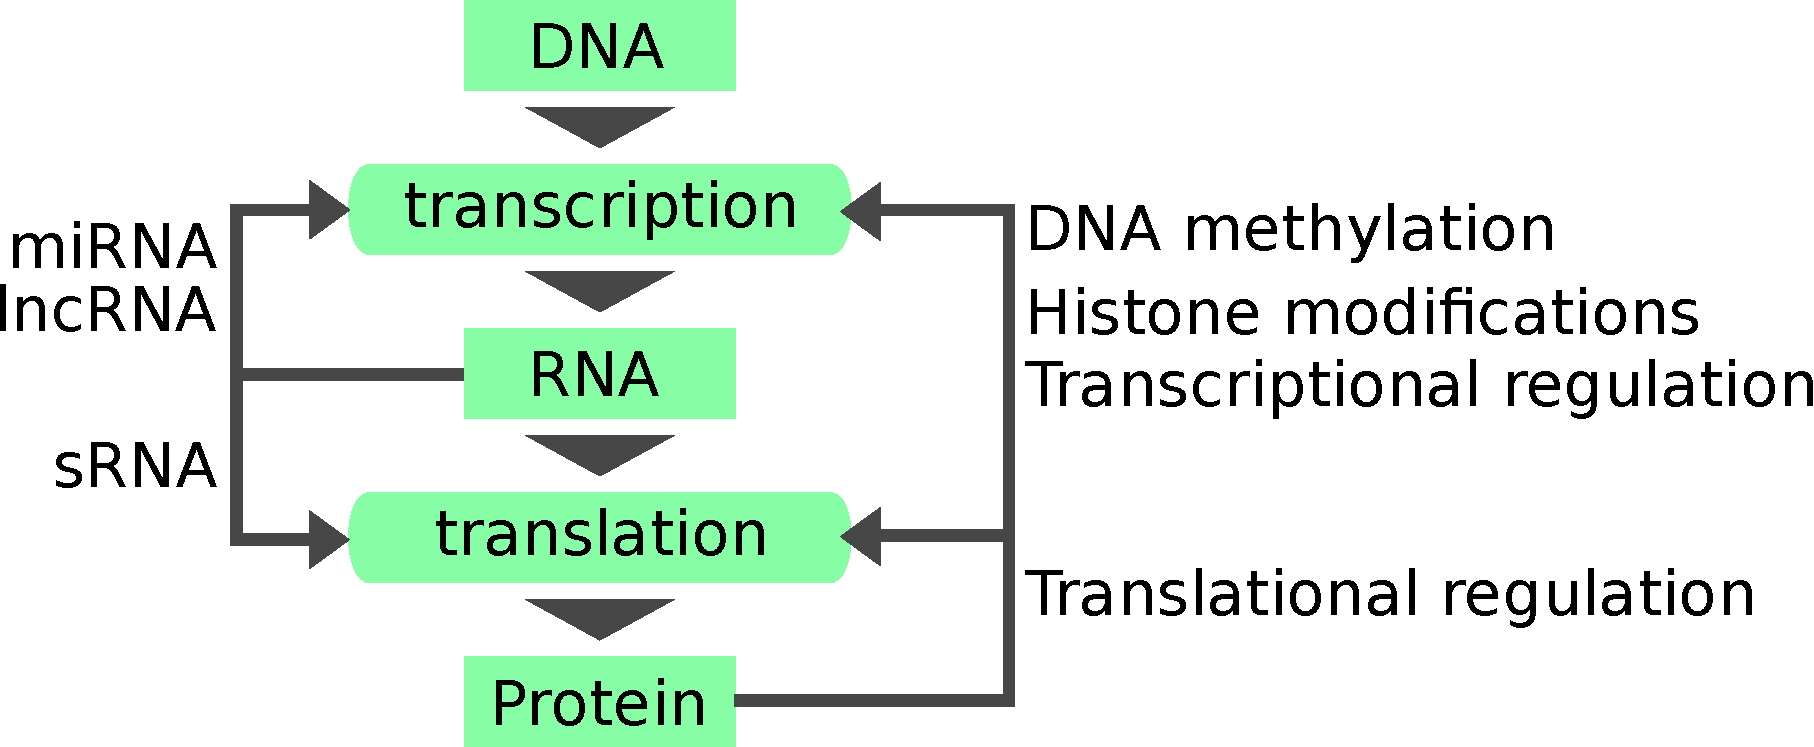
\includegraphics[width=0.8\textwidth]{Parts/Part01/gfx/central_dogma_regulation.pdf}
    \caption[Central dogma of molecular biology.]{Central dogma of molecular biology. Products and reactions from the central dogma are shown in green, with grey arrows showing some of the regulatory interactions between the different biomolecules.}
    \label{fig:01-02:central-dogma}
\end{figure}

There is now a growing area of research focusing on the development of methods that combine these layers of information. They aim to gain an integrative view of biology to better model the behaviour of molecular networks. This is done by combining "omics" datasets measuring various biomolecules, such as genetic mutations, gene expression, protein binding, histone modifications or protein abundance.

One of the main challenges is to find efficient ways to combine these informations to extract meaningful biological information. More often than not, they are analysed separately to find regions of deregulation common to the different layers. Nevertheless, there have already been attempts at fully integrating these levels of information. %MOFA, DL from Anshul Kundaje

Another challenge is the difficulty to combine different datasets due to technical heterogeneities or biological differences such as different strains or experimental conditions.
